
\chapter{Proving more complex statements}


\section{trees}

	In exercise 1.3, the last two exercises were

\begin{enumerate}
	\setcounter{enumi}{7}
	
	\item $\exists x \in \mathbb{R}: [(2x+1 = 5) \wedge (3x+3 = 5)]$
	
	\item $[\exists x \in \mathbb{R}: (2x+1 = 5)] \wedge [\exists x: (3x+3 = 5)]$
\end{enumerate}

Understanding the difference between these two statements may have been difficult for you.  Here we will introduce another way to record the logical structure of these sentences called a \textbf{syntax tree} which might be a little easier to understand (once you get the hang of it).

Statement (8) is existentially quantifying the predicate $[(2x+1 = 5) \wedge (3x+3 = 5)]$ in the variable $x$.  I will record this by having the \textbf{top level node} or \textbf{root} of the syntax tree be $\exists x \in \mathbb{R}$, drawing a single vertical \textbf{branch down} from that node and then putting the syntax tree for the predicate $[(2x+1 = 5) \wedge (3x+3 = 5)]$ below it:

\begin{center}
	\begin{forest}
		[\(\exists x \in \mathbb{R}\)[Tree for ``\({(2x+1 = 5) \wedge (3x+3 = 5)}\)'']]
	\end{forest}
\end{center}

Since the predicate $[(2x+1 = 5) \wedge (3x+3 = 5)]$ is a conjunction of the two predicates $2x+1 = 5$ and $3x+3 = 5$, the tree for this predicate will have a top level node of $\wedge$, two branches, with $2x+1 = 5$ on the left and $3x+3 = 5$ on the right:

\begin{center}
	\begin{forest}
		[\(\exists x \in \mathbb{R}\)[\(\wedge\)[\({2x+1 = 5}\)][\({3x+3 = 5}\)]]]
	\end{forest}
\end{center}

The  final \textbf{leaves} at the bottom of this tree do not contain any logical connectives or quantifiers.  Each variable appearing in the leaves can be traced back to a single quantifier which introduces the variable.

However, the syntax tree for (9) would look like:

\begin{center}
	\begin{forest}
		[\(\wedge\)[\(\exists x \in \mathbb{R}\)[\( {2x+1 = 5}\)]][\(\exists x \in \mathbb{R}\)[\( {3x+3 = 5}\)]]]
	\end{forest}
\end{center}

Note that the ``tree'' analogy is a bit strange since it is upside down!  The root is at the top, and the leaves are at the bottom!  The reason for this strange convention is that we usually like to work from top to bottom when writing on a page in English.

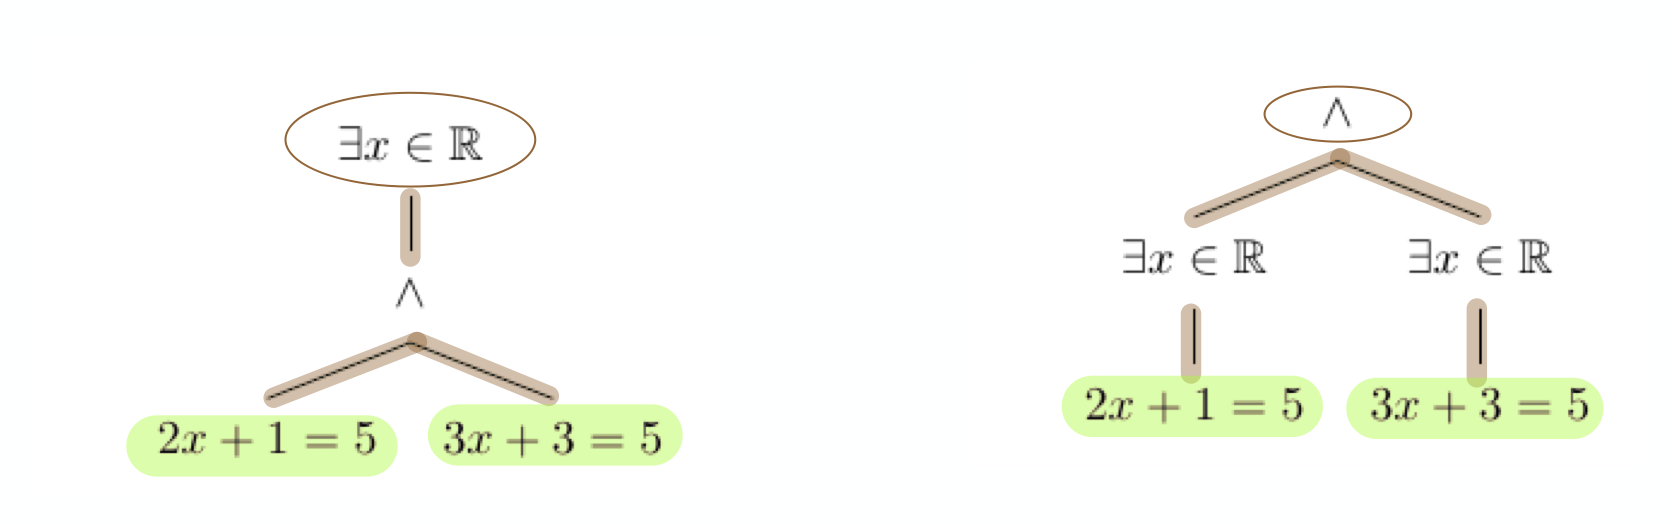
\includegraphics[scale = 0.4]{trees}

Here the root is circled, the branches are colored brown, and the leaves are colored green.

Comparing these two we see that in (8) the existential quantification of $x$ applies to both statements $2x+1 = 5$ and $3x+3  = 5$.  We would say that both instances of $x$ are within the \index{scope}\textbf{scope} of this existential quantifier.  However, in (9) the scope of the exitential quantifier on the left branch only includes the $x$ in $2x+1  = 5$, while the scope of the existential quantifier on the right branch only includes the $x$ in $3x+3 = 5$.

\begin{example}
	Assume that $P$, $Q$, and $R$ are propositions and $A$, $B$, and $C$ are predicates. The syntax tree for 
	
	\[
	\exists x :[( P \wedge A(x)) \wedge ( \forall y( B(x) \wedge C(x,y) ))]
	\]
	
	is
	
	\begin{center}
		\begin{forest}
			[\(\exists x\)[\(\wedge\)[\(\wedge\)[\(P\)][\(A(x)\)]][\(\forall y \)[\(\wedge\)[\(B(x)\)][\({C(x,y)}\)]]]]]
		\end{forest}
	\end{center}
	
	The two dimensional layout of the tree makes some features of the expression easier to parse than when we leave it as a one dimensional written expression.
\end{example}


\begin{xca}
	Build a syntax tree for each of the following statements.  Assume that $P$, $Q$, and $R$ are propositions and $A$, $B$, and $C$ are predicates.  Matching parenthesis can be a struggle:  this is part of the reason why the trees are a superior way of writing these expressions.
	
	\begin{enumerate}
		\item $\forall x:  (P \wedge \exists y (A(x,y) \wedge B(x)))$
		\item $P \wedge (Q \wedge \exists t (B(t,t)) )$
		\item $\forall x: ( \exists y (A(x,y)) \wedge \forall y (C(x,y)))$
	\end{enumerate}
\end{xca}


\begin{solutions}
	\begin{enumerate}
		\item $\forall x:  (P \wedge \exists y (A(x,y) \wedge B(x)))$
		
		\begin{center}
			\begin{forest}
				[\(\forall x\)[\(\wedge\)[\(P\)][\(\exists y\)[\(\wedge\)[\({A(x,y)}\)][\(B(x)\)]]]]]
			\end{forest}
		\end{center}
		\item $P \wedge (Q \wedge \exists t (B(t,t)) )$
		
		\begin{center}
			\begin{forest}
				[\(\wedge\)[\(P\)][\(\wedge\)[\(Q\)][\(\exists t\)[\({B(t,t)}\)]]]]
			\end{forest}
		\end{center}
		\item $\forall x: ( \exists y (A(x,y)) \wedge \forall y (C(x,y)))$
		
		\begin{center}
			\begin{forest}
				[\(\forall x\)[\(\wedge\)[\(\exists y\)[\({A(x,y)}\)]][\(\forall y\)[\({C(x,y)}\)]]]]
			\end{forest}
		\end{center}
		
	\end{enumerate}
\end{solutions}

\begin{xca}
	Consider the syntax tree
	
	\begin{center}
		\begin{forest}
			[$\forall x$[$\wedge$[$\exists y$[${A(x,y)}$]][$\forall y$[$\wedge$[$P$][${B(x,y)}$]]]]]
		\end{forest}
	\end{center}
	
	Indicate all variables which are in the scope of $\forall y$.  Then convert this syntax tree to a linear string with appropriate parentheses. 
	
\end{xca}

\begin{xca}
	The only variable within the scope of $\forall y$ is the $y$ in $B(x,y)$.
	
	We can write this proposition on one line as
	
	\[
	\forall x: (  (\exists y: ( A(x,y)))  \wedge (\forall y: ( P \wedge  B(x,y)))  )
	\]
	
\end{xca}

\subsection{Fitch style proof outlines for statements involving only quantifiers and conjunctions}

Since we already know how to make Fitch style proof outlines for existentially quantified statements, universally quantified statements, and conjunctions, we can put these together to make more complicated Fitch style proof outlines.



\section{Introduction}

We have seen that we can make the logical structure of mathematical statements clearer by translating them into statements in first order logic.  That is to say, if we declare the meaning of sentences like $p$, $q$, $r$,  and predicates like $A(x)$,  $B(x)$,  $C(x,y)$, then we can use the logical connectives $\wedge$, $\implies$, $\equivalent$, $\neg$, $\vee$ and the quantifiers $\forall$ and $\exists$ to translate mathematical statements in English into more formal and precise statements using these symbols.

For example, if we let $E(x)$ be the predicate ``$x$ is even'', then we can translate the English mathematical sentence 

{ \begin{center}
		``The product of any two even numbers is even.''
		\end{center}
}

into a symbolic form where its logical structure is more apparent:

$$
\forall x \in \Z \, \forall y \in \Z \left( E(x) \wedge E(y) \implies E(x+y) \right)
$$

or as a syntax tree:

\begin{center}
\begin{forest}
	[$\forall x \in \Z$[$\forall y \in \Z$[$\implies$[$\wedge$[$E(x)$][$E(y)$]][$E(x+y)$]]]
]
\end{forest}
\end{center}

We will see how to use this logical structure to make a ``Fitch Style Proof Outline''  for the theorem.  We will generate this outline recursively, moving down the tree.  Proving theorems in mathematics often requires considerable creativity, but that creativity often lives in the ``blank spaces'' of this outline, not in the structure of the outline itself.  For each of the five connectives, and two quantifiers, we will see how to both \textbf{use} a statement whose top level node is of that form, and how to \textbf{prove} a statement whose top level node is of that form.

By \textbf{using} a statement I mean that if we know (somehow) that the statement is true, what can we conclude from that?  By \textbf{proving} a statement I mean that if we want to argue that a statement is true, what must we do to convince someone of that?

 

\section{Top level nodes}

Let's call a statement a conjunction (or less formally an ``and statement'') if the top level node of its syntax tree is $\wedge$.

For instance 

$$
(\forall x (\exists y (A(x) \implies B(x,y))))) \wedge (\exists x, A(x))
$$

is a conjunction because its syntax tree is

\begin{center}
	\begin{forest}	
		[$\wedge$[$\forall x$[$\exists y$[$\implies$[$A(x)$][{$B(x,y)$}]]]][$\exists x$[$A(x)$]]]
		\end{forest}
	\end{center}

However, the sentence

$$
\forall x (A(x) \wedge [\exists y (A(x) \implies B(x,y))])
$$

is not a conjunction, because its top level node is a universal quantifier.

We will categorize sentences according to their top level nodes.


\begin{table}[h]
	\centering
	\begin{tabular}{c|l|l}
	Top Level Node & Formal Name & Informal Name 	\\ \hline
	$\wedge$ & Conjunction & ``and'' sentence\\ \hline
	$\implies$ & Implication & ``implies'' sentence\\ \hline
	$\equivalent$ & Biconditional & ``if and only if'' sentence\\ \hline
	$\neg$ & Negation & ``not'' sentence\\ \hline
	$\vee$ & Disjunction & ``or'' sentence\\ \hline
	$\forall$ & Universally quantified sentence & ``for all'' sentence\\ \hline
	$\exists$ & Existentially quantified sentence & ``there exists'' sentence\\ \hline
	\end{tabular}
\end{table}

 \newpage

\section{Conjunctions}

If $p$ and $q$ are two sentences, we have seen that the truth table for their conjunction is as follows:

\begin{table}[h]
	\centering
	\begin{tabular}{c|c|c}
		$p$ & $q$ & $p \wedge q$ 	\\ \hline
		F & F & F 	\\ \hline
		F & T & F 	\\ \hline
		T & F & F 	\\ \hline
		T &  T & T 	\\ \hline
	\end{tabular}
\end{table}

\subsection{Using a conjunction}  If we know that the conjunction $p \wedge q$ is true, then we know (from looking at the truth table) that both $p$ and $q$ are each true individually.  So if we know that a conjunction is true, we can use that each of its branches are also true.

In a proof, if we know that $p \wedge q$ is true, then we may cite that fact that $p$ is true or that $q$ is true whenever we want in our argument. 

\subsection{Proving a conjunction}  To show that a conjunction is true, we need to demonstrate that both $p$ is true and $q$ is true.  We will do this in our proof outline as follows:

To prove $p \wedge q$:

\begin{fitch*}
		\textrm{(Need to show $p \wedge q$ is true)}\\
		\textrm{Put a proof of $p$ here.}\\
		\textrm{Put a proof of $q$ here.}\\
		\textrm{Conclude that $p \wedge q$ is true.}\\
		\textrm{Note: If this was only part of your argument, continue with whatever other arguments you are making.}\\ \textrm{ \hphantom{Note:}From this point on you can use the fact that $p$, $q$ and $p \wedge q$ are all true.}\\
	\end{fitch*}

What does a proof of $p$ look like?  Well, usually $p$ will itself be a complicated logical statement.  So we will look at the top level node of $p$, and continue this process of constructing the proof outline recursively.

\newpage

\section{Implication}

If $p$ and $q$ are two sentences, we have seen that the truth table for the implication $p \implies q$ is:

\begin{table}[h]
	\centering
	\begin{tabular}{c|c|c}
		$p$ & $q$ & $p \implies q$ 	\\ \hline
		F & F & T 	\\ \hline
		F & T & T 	\\ \hline
		T & F & F 	\\ \hline
		T &  T & T 	\\ \hline
	\end{tabular}
\end{table}

\subsection{Using an implication}

If we know (somehow) that the implication $p \implies q$ is true, then there are two useful ways to use this knowledge in arguments.

One way is straightforward:  if we also (somehow) know that $p$ is true, then we can conclude that $q$ is true.  There is only one row of the truth table where both $p$ and $p \implies q$ are both true, and in that row $q$ is also true.

The other way is less straightforward:  if we also (somehow) know that $q$ is false, then what can we conclude?  Look at the truth table.  Are their any rows where $q$ is false and $p \implies q$ is true?  There is only one such row, and it is the row where $p$ is also false.  So if we know $p \implies q$ is true, and we know $q$ is false,  we can conclude that $p$ is also false. 

You may recall that the contrapositive of $p \implies q$ is $(\neg q) \implies (\neg p)$.  The contrapositive of an implication is equivalent to the original implication.  So really all we were saying in the last paragraph is that if we know that an implication is true, we can also use its contrapositive.

What happens if we know an implication $p \implies q$ is true, and we know that $p$ is false?  This is a sad situation to be in, because the implication is useless for making arguments.  We can see that in this case, $q$ could be true or false, so we gain no information about $q$ in this case.  Similarly, knowing that $q$ is true gives us no information about $p$.

\subsection{Proving an implication}

If we want to convince someone that an implication $p \implies q$ is true, what do we need to do?

If the hypothesis $p$ is false, then the implication is automatically true (no matter whether the conclusion $q$ is true or false).  Remember that we call this kind of implication ``vacuously true''.  

So to convince someone that an implication $p \implies q$ is true, we do not need to ever consider the case when $p$ is false.  We only have to consider what happens when $p$ is true.  If $p$ is true, then for the implication to be true we need to show that $q$ is also true.

In other words, to prove an implication $p \implies q$ we should \textbf{assume} (or pretend) that $p$ is true, and try to argue that $q$ must be true relative to that assumption.

In our proof outline, we will record the fact that we have made an \textbf{assumption} by initiating a vertical bar with an indent.  Every part of the argument within the scope of that vertical bar is made relative to the assumption (so we can always pretend that the assumption is true for those parts of the argument).  We cannot assume that the assumption is true in other places of our argument!  When we have finished proving the implication, we end the vertical bar, and unindent.

 
\newpage

So our proof outline looks like this:


	\begin{fitch*}
		\textrm{(Need to show $p \implies q$ is true)}\\
		\textrm{Assume $p$ is true.}\\
		\fa \textrm{ Argue that $q$ is true, assuming that $p$ is true}\\
		\fa \textrm{ Continue arguing that $q$ is true, still under the assumption that $p$ is true.}\\
		\fa \textrm{ Conclude that $q$ is true.}\\
		\textrm{Conclude that $p \implies q$ is true.}\\
		\textrm{Continue with the rest of your argument.  From this point forward you can use the fact that $p \implies q$ is true.}\\
	\end{fitch*}

Note:  you \textbf{cannot} use that either $p$ or $q$ are true.  We only proved that if $p$ is true, then $q$ is.  We didn't actually argue that either one was true.

\newpage

\section{Recursion in the proof outline}

Before we explore strategies for using and proving the other logical operators and quantifiers we will pause to understand the recursive nature of the proof outline.  At this point, we only have $\wedge$ and $\implies$, so let us see what the proof outline for a sentence which only uses these two connectives looks like.

Say we wanted to argue that the following English sentence is true:

\begin{center}
		``If Superman is strong and quick, then he can save both Batman and Robin''
	\end{center}

Let us formalize this as follows:

\begin{align*}
	S &= \textrm{``Superman is strong''}\\
	Q&= \textrm{``Superman is quick''}\\
	B &= \textrm{``Superman can save Batman"}\\
	R &= \textrm{``Superman can save Robin''}
\end{align*}

Then the symbolic translation of our original sentence is

$$
S \wedge Q \implies B \wedge R
$$

whose syntax tree is

\begin{center}
\begin{forest}
	[$\implies$[$\wedge$[S][Q]][$\wedge$[B][R]]]
	\end{forest}
\end{center}

Let us see how to create a Fitch Style proof outline for this sentence.

This is an implication, so we know that we should assume the hypothesis and try to argue the conclusion.

\begin{fitch*}
	\textrm{Assume $S \wedge Q$}\\
	\fa \textrm{Try to prove $B \wedge R$}
	\end{fitch*}

 

How do we try to prove $B \wedge R$?  We follow the proof outline for $\wedge$!

\begin{fitch*}
	\textrm{Assume $S \wedge Q$ is true.}\\
	\fa \textrm{Prove $B$ is true.}\\
	\fa \textrm{Prove $R$  is true.}\\
	\fa \textrm{Conclude $B \wedge R$ is true.}
\end{fitch*}

During the proof of $B$ and $R$ we are allowed to assume $S \wedge Q$ is true, which means we can freely utilize the facts that $S$ is true and $Q$ is true in our argument.

If it turns out that proving $B$ is true is equivalent to some more complicated fact which must be argued (``Batman can be saved if either someone can lift a bus off of him, or if they can run to the Batmobile fast enough to retrieve his med kit''), then you would continue to recursively fill in the proof outline.

Let us now return our attention to the other logical operators and quantifiers.

\newpage

\section{Biconditional}

We know that $p \equivalent q \equiv (p \implies q) \wedge (q \implies p)$.  Since we already know how to both use and prove conjunctions and implications, we already (in principle) know how to use and prove biconditionals!  Let's spell out the details.

\subsection{Using an biconditional} 

If we know (somehow) that the biconditional $p \equivalent q$ is true, then we also know that $(p \implies q) \wedge (q \implies p)$ is true.  So we can use that $p \implies q$ is true, and that $q \implies p$ is true.   Further breaking these down we know that

\begin{itemize}
		\item If $p$ is true, then $q$ must also be true.
		\item If $q$ is true, then $p$ must also be true.
		\item If $p$ is false, then $q$ must also be false.
		\item If $q$ is false, then $p$ must also be false. 
	\end{itemize}

The last two items follow from the contrapositives of the two implications.

Note:  we have essentially written down the entire truth table!  Every possible bit of knowledge about either $p$ or $q$ is useful if you know that the biconditional is true.  This was not the case for conjunction or implication.

\subsection{Proving an equivalence}

If we want to convince someone that $p \equivalent q$ is true, then we will just follow the Fitch style proof outline for $(p \implies q) \wedge (q \implies p)$.

\begin{fitch}
		\textrm{ Assume $p$ is true.}\\
		\fa \textrm{Argue that $q$ is true.}\\
		\textrm{Conclude that $p \implies q$ is true}\\
		\textrm{Assume $q$ is true.}\\
		\fa \textrm{Argue that $p$ is true.}\\
		\textrm{Conclude that $q \implies p$ is true.}\\
		\textrm{Conclude that $p \equivalent q$ is true.}
	\end{fitch}

Here on lines 1 and 2, we are arguing that $p \implies q$ is true.  On lines 4 and 5 we are arguing that $q \implies p$ is true.  Since we know that both $p \implies q$ and $q \implies p$ are true, we can conclude on line 7 that $(p \implies q) \wedge (q \implies p)$ is true, which means that $p \equivalent q$ is true.

Note:  Sometimes mathematicians will refer to lines 1 and 2 as the ``forward" or ``only if" part of the argument, and lines 4 and 5 as the ``backward'' or ``if'' part of the argument.  These names make sense because the implication arrows are either pointing forward from $p$ to $q$, or backwards from $q$ to $p$.  If we write ``$p$ if and only if $q$'', then ``$p$ only if $q$'' represents $p \implies q$ and ``$p$ if $q$'' represents $q \implies p$.

It is a very common mistake for students to forget the backward part of the argument when proving a biconditional. 

\newpage

\section{Negation}

\subsection{Using a negation}

If we know (somehow) that $\neg p$ is true, then we know $p$ is false.

Also if we know (somehow) that $\neg p$ is false, then we know that $p$ is true.

\subsection{Proving a negation}

There is a subtle asymmetry in the proof strategies we have presented so far.  We have always only been concerned with showing that a statement is true, and we have not focused on how to show that a statement is false.

This presents us with difficulties when we come to negation:  to prove that $\neg p$ is true, it seems we must argue that $p$ is false.  However, we have not discussed any strategies at all for showing that a statement is false!  So our recursive approach to constructing a proof outline seems to break down here.  We could solve this by going back and also giving proof outlines for how to show that each kind of statement is false, but we will not do this.

Observe that $(p \implies F) \equiv \neg p$:

\begin{table}[h]
	\centering
	\begin{tabular}{c|c|c}
		$p$ & $p \implies F$ & $\neg p$ 	\\ \hline
		F & T & T 	\\ \hline
		T & F & F
	\end{tabular}
\end{table}

In fact, some mathematicians like to define $\neg p$ as $p \implies F$!    Thinking of negation this way means that to prove that $\neg p$ is true, we do not need to argue that $p$ is false.  Instead we just argue that $p \implies F$ is true.

So our proof strategy for negation looks like this:

\begin{fitch*}
	\textrm{Assume $p$}\\
	\fa \textrm{Argue $F$.}\\
	\textrm{Conclude $\neg p$}
	\end{fitch*}

Often when we ``argue $F$'', we will be reaching an \textrm{absurdity}, i.e. a statement which must be false for purely logical reasons.  So we might assume $p$, make some arguments relative to that assumption, and eventually conclude something like ``$n$ is an integer and $n$ is not an integer'', or some other statement which must be false.

 
\newpage

\section{Disjunction}

We have saved the trickiest connective for last.  Let us recall the truth table for disjunction:

\begin{table}[h]
	\centering
	\begin{tabular}{c|c|c}
		$p$ & $q$ & $p \vee q$ 	\\ \hline
		F & F & F 	\\ \hline
		F & T & T \\ \hline
		T & F & T \\ \hline
		T & T & T
	\end{tabular}
\end{table}

\subsection{Using a disjunction}

If you (somehow) know that the disjunction $p \vee q$ is true, then either $p$ is true, $q$ is true, or both are true.  However, we do not know which!  So we will need to break our argument into cases:  we need to show that our argument holds in the case that $p$ is true, and we also need to show that our argument holds in the case that $q$ is true.

If you are trying to argue that some statement $r$ follows from $p \vee q$, then you are really trying to show that $p \vee q \implies r$.  I urge you to confirm the fact that

$$
(p \vee q) \implies r \equiv  (p \implies r) \wedge (q \implies r)
$$

by making a truth table.

So when you are trying to argue that $r$ is true, and you know that $p \vee q$ is true, your argument should look like this:

\begin{fitch}
		\textrm{Case 1:  Assume $p$ is true.}\\
		\fa \textrm{Argue $r$ is true.}\\
		\textrm{Case 2:  Assume $q$ is true.}\\
		\fa \textrm{Argue $r$ is true.}\\
		\textrm{Since in either case, $r$ is true, and we know $p \vee q$ is true, we can conclude that $r$ is true.}
	\end{fitch}

\newpage

\subsection{Proving a disjunction}

There are four ways to prove a disjunction:
\begin{enumerate}
		\item Prove that $p$ is true.
		\item Prove that $q$ is true.
		\item Prove that $(\neg p) \implies q$ is true.
		\item Prove that $(\neg q) \implies p$ is true. 
	\end{enumerate}

Methods 1 and 2 are the best way to prove a disjunction.  You will often end up using these strategies as part of a case analysis:  in some cases $p$ will be true, and in other cases $q$ will be true.  However, you will be able to show that either $p$ or $q$ is true in all cases, and hence establish $p \vee q$.  

Sometimes statements which are disjunctions are embedded within the scope of some quantifier, and one statement or the other is true depending on the value of a variable.  For instance, the following is a basic theorem of number theory called Euclid's Lemma:



\begin{theorem}[Euclid's Lemma]
		For any prime number $p$,  and for any integers $a$ and $b$, if $p$ divides $ab$, then $p$ divides $a$ or $p$ divides $b$.
	\end{theorem}

We will definitely not be able to prove that if a prime divides a product, then it must divide the first factor!  

In these sorts of situations we will use strategy 3 or 4 when proving a disjunction.

Note:  When making ``proof outlines'' for \textbf{abstract} sentences (where you do not know the meaning of the sentences and predicates $p$, $q$, $r$, $A(x)$, $B(x,y)$, etc), then you should use method 3 or 4 since you will not know which disjunct to prove.

I urge you to make a truth table for $p$, $q$, $p \vee q$, and $(\neg p) \implies q$ to see that $p \vee q \equiv (\neg p) \implies q$.  This equivalence is a very important thing for us to understand about disjunctions when we are proving theorems.

It should also make ``intuitive sense''.  To argue that either $p$ or $q$ is true, it should be enough to argue that if you know (somehow) that $p$ is false, then you should be able to argue that $q$ is true.

For instance, the sentence 

\begin{quote}
		Either you do your chores or you will be grounded.
	\end{quote}

is equivalent to the sentence

\begin{quote}
		If you do not do your chores, then you will be grounded.
	\end{quote}

Each of these strategies has a proof outline, so you will need to be judicious about which to employ in a given situation.

Here are the corresponding proof outlines:

\begin{enumerate}
		\item
	
	\begin{fitch*}
		\textrm{Argue $p$}\\
		\textrm{Conclude $p \vee q$}
	\end{fitch*}
		\item
	
	\begin{fitch*}
		\textrm{Argue  $q$}\\
		\textrm{Conclude $p \vee q$}
	\end{fitch*}
	\item
	
\begin{fitch*}
	\textrm{Assume $\neg p$}\\
	\fa \textrm{Argue $q$}\\
	\textrm{Conclude $p \vee q$}
	\end{fitch*}

	\item

\begin{fitch*}
	\textrm{Assume $\neg q$}\\
	\fa \textrm{Argue $p$}\\
	\textrm{Conclude $p \vee q$}
\end{fitch*}
\end{enumerate}

\newpage

\section{Making Fitch style proof outlines for unquantified sentences }

We now have the tools to make Fitch style proof outlines for any sentence which doesn't have a quantifier.  Let's see how that works for some complicated sentences before moving on to quantifiers.

Let's make a Fitch style proof outline for the following sentence:

$$
(p \vee q) \implies [(\neg s) \wedge t]
$$

I will do this in considerable detail.  Let us start by giving the syntax tree for this sentence:

\begin{center}
	\begin{forest}
			[$\implies$[$\vee$[$p$][$q$]][$\wedge$[$\neg$[$s$]][$t$]]]
		\end{forest}
\end{center}

This is an implication, so our outline will look like this:

\begin{fitch*}
	\textrm{Assume $p \vee q$}\\
	\fa \textrm{Argue that $(\neg s) \wedge t$ is true.}\\
	\textrm{Conclude that $(p \vee q) \implies [(\neg s) \wedge t]$ is true.}
\end{fitch*}

 

Now we need to replace ``Argue that $(\neg s) \wedge t$ is true'' with its Fitch style proof outline!

\begin{fitch*}
	\textrm{Assume $p \vee q$}\\
	\fa \textrm{Argue $\neg s$}\\
	\fa \textrm{Argue $t$}\\
	\fa \textrm{Conclude that $(\neg s) \wedge t$ is true.}\\
	\textrm{Conclude that $(p \vee q) \implies [(\neg s) \wedge t]$ is true.}
\end{fitch*}


Finally, we must replace ``Argue $\neg s$" with its proof outline.

\begin{fitch*}
	\textrm{Assume $p \vee q$.}\\
	\fa \textrm{Assume $s$.}\\
	\fa \fa \textrm{Argue $F$.}\\
	\fa \textrm{Conclude $\neg s$.}\\
	\fa \textrm{Argue $t$.}\\
	\fa \textrm{Conclude that $(\neg s) \wedge t$ is true.}\\
	\textrm{Conclude that $(p \vee q) \implies [(\neg s) \wedge t]$ is true.}
\end{fitch*}

\newpage

\section{Universal Quantification}

\subsection{Using a universally quantified sentence}

If you know (somehow) that the sentence $\forall x \in \mathcal{U}, P(x)$ is true then if you have a particular element $a$ of your universe of discourse $\mathcal{U}$, then you also know that $P(a)$ is true.  This is sometimes called by the fancy name of ``Universal Elimination".

For example, if you know that ``For every integer $x$, $6x$ is even'', and at some point in your argument you need that $6*101$ is even, you can  quote the theorem using $x = 101$ to support your argument.

\subsection{Proving a universally quantified sentence}

If your universe of discourse is finite, then you can prove $\forall x P(x)$ by just checking each element.  If $P(x)$ is true for every single input $x$, then the universally quantified statement is true.  If there is even a single value of $x$ which makes $P(x)$ false, then $\forall x P(x)$ is false.

However, if your universe of discourse is infinite, we cannot prove a universally quantified sentence by manually checking all of the cases.  

What we do is to choose a ``generic'' or ``arbitrary'' element of our universe of discourse, give it a name, and then argue that $P$ is true for that generic element.

Say you want to prove that ``Everyone who has a beard gets crumbs in it sometimes''.  This could be argued by saying ``Imagine someone who has a beard. Let's just call them Bob.  Then [arguments].  So we can conclude that Bob sometimes gets crumbs in their beard.  There was nothing special about Bob.  Therefore everyone with a beard sometimes gets crumbs in it''.

The Fitch style proof outline for universally quantified sentences is 

\begin{fitch*}
	\textrm{(To prove $\forall x P(x)$)}\\
	\textrm{Let $a$ be an arbitrary element of the universe of discourse.}\\
	\textrm{Prove $P(a)$}.\\
	\textrm{Conclude $\forall x P(x)$.}
\end{fitch*}

Note:  it is important to avoid variable name conflicts!  If you have already named a variable $a$ earlier in the argument, and that name is still ``in use'', then reusing it can cause real confusion.  Imagine you were telling a story about your friends and you said

``My one friend, lets just call him Joe, started going out with my other friend, lets just call him Keith.  What Joe didn't know is that Keith was going out with my other friend.  Let's just call this other friend Joe.  So Joe found out about Joe, and you can imagine the kind of upset that caused''.

Accidentally calling two different friends by the same name has caused the potential for real confusion in your story.

\newpage

\section{Existential Quantification}

\subsection{Using Existentially Quantified Sentences}

If you know (somehow) that the sentence $\exists x \in \mathcal{U}, P(x)$ is true, then you know there is at least one value which makes the predicate true, but you do not know which one.  So you can choose one of the things which makes it true, and give it a name (like $a$) so you can refer to it later, but you may not make any other assumptions about the nature of $a$.

A typical example of this is that if you know that $a$ is odd, that means (by definition) that $\exists k \in \mathbb{Z}, a=2k+1$.  So you can choose such an element, and call it (say) $m$.  Then you know that $a=2m+1$, but you do not know anything else about $m$.  

Similar remarks about variable conflicts apply here:  do not choose a variable name which is already is use.  If $b$ is an even number, and you already know $a=2m+1$, do not say $b = 2m$, because you are using the same variable $m$ to reference two potentially different constants.  Instead choose a variable name you have not used yet, like $n$.  So if we know $a$ is odd and $b$ is even, we can declare integers $m$ and $n$ so that $a=2m+1$ and $b = 2n$.

\subsection{Proving Existentially Quantified Sentences}

To prove an existentially quantified sentence you need to find a candidate element $a$ of the universe of discourse for which you believe that $P(a)$ is true, and then supply a proof that $P(a)$ is actually true.

The Fitch style proof outline for $\exists x P(x)$ looks like this:

\begin{fitch*}
		\textrm{(To prove $\exists x P(x)$)}\\
		\textrm{Construct a candidate $a$ in the universe of discourse.}\\
		\textrm{Give a proof that $P(a)$ is true.}\\
		\textrm{Conclude $\exists x P(x)$.}
\end{fitch*} 

Note:  Existentially quantified sentences are a bit funny.  The construction of $a$ is often more important than the statement that $a$ exists.  It is much more useful to know that $1729$ is an integer which is expressible as sum of two cubes in two different ways ($1729 = 1^3+12^3 = 9^3+10^3$ ) than it is to know that there is some integer which is expressible as a sum of two cubes in two different ways.

 \newpage
 
\section{Summary Table}

\begin{table}[h]
	\centering
	\begin{tabular}{c?p{5 cm}?p{4 cm}}
		Top Level Node & How to use it if it is true & How to prove that it is true	\\ 
		$p \wedge q$ & You also know that $p$ is true and $q$ is true.  & Argue $p$ is true.  Then argue $q$ is true. \\ \hline
		$p \implies q$ & If you also know $p$ is true, then you know $q$ is true. & \begin{fitch*}
			\textrm{Assume $p$ is true.} \\
			\fa \textrm{Argue that $q$ is true.}
		\end{fitch*}\\ \hline
		$p \equivalent q$ & If you know the truth value of one, then the truth value of the other is identical. &  
		\begin{fitch*}
			\textrm{Assume $p$ is true.} \\
			\fa \textrm{Argue that $q$ is true.}\\
			\textrm{Assume $q$ is true.} \\
			\fa \textrm{Argue that $p$ is true.}
		\end{fitch*}
		\\ \hline
		$\neg p$ & $p$ is false. &  
		\begin{fitch*}
			\textrm{Assume $p$}\\
			\fa \textrm{Argue $F$}
		\end{fitch*}
		\\ \hline
		$p \vee q$ & If you are trying to argue $r$ is true, then you must split your argument into cases.
		\begin{fitch*}
			\textrm{Case 1: Assume $p$ is true.}\\
			\fa \textrm{Argue $r$ is true.}\\
			\textrm{Case 2:  Assume $q$ is true.}\\
			\fa \textrm{Argue $r$ is true.}
		\end{fitch*}
		&  Argue $p$ is true.
		
		\medskip
		
		OR
		
		\medskip
		
		Argue $q$ is true.
		
		\medskip
		
		OR
		
		\begin{fitch*}
			\textrm{Assume $\neg p$ is true.}\\
			\fa \textrm{Argue $q$ is true. }
		\end{fitch*}
		
		OR 
		
		\begin{fitch*}
			\textrm{Assume $\neg q$ is true.}\\
			\fa \textrm{Argue $p$ is true. }
		\end{fitch*}
		
		\\ \hline
		$\forall x, A(x)$ & If $t$ is any element of the universe of discourse, you know that $A(t)$ is true. &  Let $x_1$ be an arbitrary element of the universe of discourse, and argue that $A(x_1)$ is true. \\ \hline
		$\exists x, B(x)$ & You know that there is at least one (and potentially only one) element of your universe of discourse which makes $B$ true.  Pick one and call it $x_1$.  You may freely use that $B(x_1)$ is true in your argument. &  You need to come up with a candidate $x_1$ for which you think $B(x_1)$ is true.  Often, this will be a formula in terms of previously declared variables.  Then argue that $B(x_1)$ really is true.
	\end{tabular}
\end{table}

\newpage


\section{Putting it all together!}

We can now construct proof outlines for arbitrary sentences!  For the rest of this course we will be focused on proving theorems about mathematical objects of interest.  Here is a sample of the kinds of theorems we will prove:

\begin{enumerate}
		\item 	If $x$ is a real number then $x^2 = 1$ if and only if $x=1$ or $x=-1$.
		\item If $a$ is odd, and $b$ is odd, then $a+b$ is even.
		\item Let $p$, $a$, $b$ be integers.  If $p$ is prime, and $p$ is a factor of $ab$, then either $p$ is a factor of $a$ or $p$ is a factor of $b$.
		\item For every positive real number $x$, there is real number $y$ so that if $t$ is another real number and $0<t<y$ then $0<t^2<x$.
\end{enumerate}


Let's create proof outlines for each of these.  You may or may not be able to fill in the details of these outlines (to get a full proof), but that is not the point right now:  we just want to feel confident that we know what we should be trying to do when proving these statements, not how to actually prove them yet.

\medskip

\begin{theorem}
		If $x$ is a real number then $x^2 = 1$ if and only if $x=1$ or $x=-1$.
	\end{theorem}

\begin{proof}[Proof outline]
	
	You probably learned this theorem in high school algebra.  It is the real reason you put $\pm$ signs when you take square roots.  Even though you know this theorem is true, and use it frequently, you have probably never seen a proof.  
	
	Let's prove it!

We can translate this statement into symbolic logic as follows:

\[
\forall x \in \mathbb{R} [ ({x^2 = 1}) \iff [({x=1}) \vee ({x=-1})] ]
\]

The syntax tree is

\begin{center}
		\begin{forest}
				[\(\forall x \in \mathbb{R}\)[\(\iff\)[\({x^2 = 1}\)][\(\vee\)[\({x=1}\)][\({x=-1}\)]]]]
			\end{forest}
	\end{center}


To construct the proof outline, we move recursively down the tree.  I will do this in \textbf{excruciating} detail.  You want to get to the point where you can easily write down the proof outline without working methodically like this.

The top level node is a universal quantifier, so we start with that proof outline.

\begin{fitch}
	\textrm{Let $a \in \mathbb{R}$ be arbitrary.}\\
	\textrm{Argue $({a^2 = 1}) \iff [({a=1}) \vee ({a=-1})]$ is true. }
	\end{fitch}

The statement in line 2 is a biconditional, so to prove it we need to argue the forwards and backwards implications:

\begin{fitch}
	\textrm{Let $a \in \mathbb{R}$ be arbitrary.}\\
	\textrm{Assume $a^2 = 1$ is true.}\\
	\fa \textrm{Argue $(a=1) \vee (a=-1)$ is true.}\\
	\textrm{Assume $(a=1) \vee (a=-1)$ is true.}\\
	\fa \textrm{Argue $a^2 = 1$ is true.}
\end{fitch}

To argue that disjunction in line 3 is true, we will assume the negation of one disjunct and try to argue the other is true.

\begin{fitch}
	\textrm{Let $a \in \mathbb{R}$ be arbitrary.}\\
	\textrm{Assume $a^2 = 1$ is true.}\\
	\fa \textrm{Assume $a \neq 1$}\\
	\fa \fa \textrm{Argue that $a=-1$}\\
	\textrm{Assume $(a=1) \vee (a=-1)$ is true.}\\
	\fa \textrm{Argue $a^2 = 1$ is true.}
\end{fitch}

To argue that $a^2=1$ in line 6, we will need to \textbf{use} the disjunction we assumed in line 5.  This is where we use a case analysis:

\begin{fitch}
	\textrm{Let $a \in \mathbb{R}$ be arbitrary.}\\
	\textrm{Assume $a^2 = 1$ is true.}\\
	\fa \textrm{Assume $a \neq 1$}\\
	\fa \fa \textrm{Argue that $a=-1$}\\
	\fa \textrm{Conclude that $(a=1) \vee (a=-1)$ is true.}\\
	\textrm{Conclude that $(a^2 = 1) \implies (a=1) \vee (a=-1)$ is true.}\\
	\textrm{Assume $(a=1) \vee (a=-1)$ is true.}\\
	\fa \textrm{Case 1:  Assume $a = 1$ is true.}\\
	\fa \fa \textrm{Argue $a^2 = 1$ is true.}\\
	\fa \textrm{Case 2:  Assume $a = -1$ is true.}\\
	\fa \fa \textrm{Argue $a^2 = 1$ is true.}\\
	\fa \textrm{Conclude $a^2 = 1$ is true.}\\
	\textrm{Conclude that $[(a=1) \vee (a=-1)] \implies (a^2 = 1)$ is true.}\\
	\textrm{Conclude that $[(a=1) \vee (a=-1)] \iff (a^2 = 1)$ is true.}\\
	\textrm{Conclude that $\forall x \in \mathbb{R} [ ({x^2 = 1}) \iff [({x=1}) \vee ({x=-1})] ] $}
\end{fitch}


This is the complete proof outline!

We can now fill in the remaining arguments to have a proof of the theorem:

\begin{fitch}
	\textrm{Let $a \in \mathbb{R}$ be arbitrary.}\\
	\textrm{Assume $a^2 = 1$ is true.}\\
	\fa \textrm{Assume $a \neq 1$}\\
	\fa \fa \textrm{Since $a^2 = 1$, we have $a^2-1 = 0$}\\
	\fa \fa \textrm{So $(a-1)(a+1) = 0$}\\
	\fa \fa \textrm{Since $a \neq 1$, $a-1 \neq 0$, and we can divide by it.}\\
	\fa \fa \textrm{So $a+1 = 0$}\\
	\fa \fa \textrm{So $a = -1$}\\
	\fa \textrm{Conclude that $(a=1) \vee (a=-1)$ is true.}\\
	\textrm{Conclude that $(a^2 = 1) \implies (a=1) \vee (a=-1)$ is true.}\\
	\textrm{Assume $(a=1) \vee (a=-1)$ is true.}\\
	\fa \textrm{Case 1:  Assume $a = 1$ is true.}\\
	\fa \fa \textrm{Then $a^2 = 1^2$, so $a^2 = 1$}\\
	\fa \textrm{Case 2:  Assume $a = -1$ is true.}\\
	\fa \fa \textrm{Then $a^2 = (-1)^2$, so $a^2 = 1$.}\\
	\fa \textrm{Conclude $a^2 = 1$ is true.}\\
	\textrm{Conclude that $[(a=1) \vee (a=-1)] \implies (a^2 = 1)$ is true.}\\
	\textrm{Conclude that $[(a=1) \vee (a=-1)] \iff (a^2 = 1)$ is true.}\\
	\textrm{Conclude that $\forall x \in \mathbb{R} [ ({x^2 = 1}) \iff [({x=1}) \vee ({x=-1})] ] $}
\end{fitch}

	\end{proof}

\begin{theorem}
	If $a$ is odd, and $b$ is odd, then $a+b$ is even.
	\end{theorem}

\begin{proof}[Proof Outline]
	We can translate this statement into symbolic logic as follows:
	
	$$
	\forall a \in \Z \,\forall b \in \Z ((\textrm{$a$ is odd} \wedge \textrm{$b$ is odd}) \implies \textrm{$a+b$ is even})
	$$

The syntax tree is

\begin{center}
	\begin{forest}
			[$\forall a \in \Z$[$\forall b \in \Z$[$\implies$ [$\wedge$[$a$ is odd][$b$ is odd]][$a+b$ is even]]]]
		\end{forest}
	\end{center}

To construct the proof outline, we move recursively down the tree.  Just like in the last proof, I will do this very methodically so that you can benefit from seeing the process in detail.

The top level node is a universal quantifier, so we start with that proof outline.

\begin{fitch}
	\textrm{Let $a_1 \in \Z$ be arbitrary.}\\
	\textrm{Prove $\forall b \in \Z ((\textrm{$a_1$ is odd} \wedge \textrm{$b$ is odd}) \implies \textrm{$a_1+b$ is even})$}\\
	\textrm{Conclude $\forall a \in \Z \,\forall b \in \Z ((\textrm{$a$ is odd} \wedge \textrm{$b$ is odd}) \implies \textrm{$a+b$ is even})$}
	\end{fitch} 

How do we argue line 2?  We replace the statement to be proved in line 2 with its proof outline!  Line 2 is also a universally quantified sentence, so we use the corresponding proof outline (being careful not to create variable name conflicts).

\begin{fitch}
	\textrm{Let $a_1 \in \Z$ be arbitrary.}\\
	\textrm{Let $b_1 \in \Z$ be arbitrary.}\\
	\textrm{Prove $(\textrm{$a_1$ is odd} \wedge \textrm{$b_1$ is odd}) \implies \textrm{$a_1+b_1$ is even}$}\\
	\textrm{Conclude $\forall b \in \Z ((\textrm{$a_1$ is odd} \wedge \textrm{$b$ is odd}) \implies \textrm{$a_1+b$ is even})$}\\
	\textrm{Conclude $\forall a \in \Z \,\forall b \in \Z ((\textrm{$a$ is odd} \wedge \textrm{$b$ is odd}) \implies \textrm{$a+b$ is even})$}
\end{fitch} 

Now line 3 is an implication

\begin{fitch}
	\textrm{Let $a_1 \in \Z$ be arbitrary.}\\
	\textrm{Let $b_1 \in \Z$ be arbitrary.}\\
	\textrm{Assume $( \textrm{$a_1$ is odd} \wedge \textrm{$b_1$ is odd}) $}\\
	\fa \textrm{Argue that $a_1+b_1$ is even.}\\
	\textrm{Conclude that $(\textrm{$a_1$ is odd} \wedge \textrm{$b_1$ is odd}) \implies \textrm{$a_1+b_1$ is even}$}\\
	\textrm{Conclude $\forall b \in \Z ((\textrm{$a_1$ is odd} \wedge \textrm{$b$ is odd}) \implies \textrm{$a_1+b$ is even}$}\\
	\textrm{Conclude $\forall a \in \Z \,\forall b \in \Z ((\textrm{$a$ is odd} \wedge \textrm{$b$ is odd}) \implies \textrm{$a+b$ is even}$}
\end{fitch} 

Each of these proof outlines is useful as a different level of ``granularity" of the proof.  Maybe this proof outline is enough for me to get to work.  Maybe not, and I need more detail.  If I need more detail, I could spell out what ``odd'' and ``even'' mean, and continue to expand the proof outline further.  For instance  ``$a_1+b_1$ is even'' means $\exists n \in \Z, \, a_1+b_1 = 2n$.

\begin{fitch}
	\textrm{Let $a_1 \in \Z$ be arbitrary.}\\
	\textrm{Let $b_1 \in \Z$ be arbitrary.}\\
	\textrm{Assume $( \textrm{$a_1$ is odd} \wedge \textrm{$b_1$ is odd}) $}\\
	\fa \textrm{Argue that $\exists n \in \Z, \, a_1+b_1 = 2n$ is true.}\\
	\textrm{Conclude that $(\textrm{$a_1$ is odd} \wedge \textrm{$b_1$ is odd}) \implies \textrm{$a_1+b_1$ is even}$}\\
	\textrm{Conclude $\forall b \in \Z ((\textrm{$a_1$ is odd} \wedge \textrm{$b$ is odd}) \implies \textrm{$a_1+b$ is even}$}\\
	\textrm{Conclude $\forall a \in \Z \,\forall b \in \Z ((\textrm{$a$ is odd} \wedge \textrm{$b$ is odd}) \implies \textrm{$a+b$ is even}$}
\end{fitch} 

Then we could further expand line 4 by using the proof outline for existential quantification.  Actually constructing this $n$ would require us to use what we know about $a_1$ and $b_1$.

Here is a complete proof outline:

\begin{fitch}
	\textrm{Let $a_1 \in \Z$ be arbitrary.}\\
	\textrm{Let $b_1 \in \Z$ be arbitrary.}\\
	\textrm{Assume $( \textrm{$a_1$ is odd} \wedge \textrm{$b_1$ is odd}) $}\\
	\fa \textrm{We know $\exists k, \, a_1 = 2k+1$.  Let $k_1\in \Z$ satisfy $a_1 = 2k_1+1$  }.\\
	\fa \textrm{We know $\exists k, \, b_1 = 2k+1$.  Let $k_2\in \Z$ satisfy $a_1 = 2k_2+1$  }.\\
	\fa \textrm{Choose $n$ somehow, and verify that $a_1+b_1 = 2n$}.\\
	\textrm{Conclude that $(\textrm{$a_1$ is odd} \wedge \textrm{$b_1$ is odd}) \implies \textrm{$a_1+b_1$ is even}$}\\
	\textrm{Conclude $\forall b \in \Z ((\textrm{$a_1$ is odd} \wedge \textrm{$b$ is odd}) \implies \textrm{$a_1+b$ is even}$}\\
	\textrm{Conclude $\forall a \in \Z \,\forall b \in \Z ((\textrm{$a$ is odd} \wedge \textrm{$b$ is odd}) \implies \textrm{$a+b$ is even}$}
\end{fitch} 
 
 
This proof outline is now only a few steps away from being a full proof of the theorem.  The entire structure of the argument has been generated ``automatically'', and the only place left for our creative efforts is to figure out how to choose $n$.  There is no magic recipe for that:  there is a tiny spark of creativity needed.  At this point you should pause and play on some scratch paper to figure out what $n$ should be.  Note:  while we are playing, we don't have to be logical.  We are just trying to generate ideas.  We can be as wild as we want to be.  Once that wild, illogical play generates an idea, we then need to be logical and precise in confirming that the idea works.

Here is what my play might look like:

\begin{itemize}
		\item Hmm, I need to show  $a_1+b_1$ equals something, but I don't know what $n$ is yet.  I am trying to choose an $n$ which works.
		\item What do I know about $a_1$ and $b_1$?
		\item Pretty much the only thing I know is that $a_1 = 2k_1+1$ and $b_1 = 2k_2+1$.
		\item Okay, so let me add those together.
		\item $(2k_1+1)+(2k_2+1) = 2k_1+2k_2+2$.
		\item Hmm, I want 2 times something, but what I have is just a bunch of  stuff added together.
		\item OH! I could undistribute the common factor of 2!
		\item So $a_1+b_1 = 2(k_1+k_2+1)$.
		\item So if I choose $n = k_1+k_2+1$, I should be able to make the argument work.
	\end{itemize}

Now we can fill in the details, and produce a full proof of the theorem:

\begin{fitch}
	\textrm{Let $a_1 \in \Z$ be arbitrary.}\\
	\textrm{Let $b_1 \in \Z$ be arbitrary.}\\
	\textrm{Assume $( \textrm{$a_1$ is odd} \wedge \textrm{$b_1$ is odd}) $}\\
	\fa \textrm{We know $\exists k, \, a_1 = 2k+1$.  Let $k_1\in \Z$ satisfy $a_1 = 2k_1+1$  }.\\
	\fa \textrm{We know $\exists k, \, b_1 = 2k+1$.  Let $k_2\in \Z$ satisfy $a_1 = 2k_2+1$  }.\\
	\fa \textrm{Choose $n = k_1+k_2+1$.  Note that $n \in \Z$}\\
	\fa \textrm{Then $a_1+b_1 = (2k_1+1)+(2k_2+1)$}.\\
	\fa \textrm{So $a_1+b_1 = 2k_1+2k_2+2$}\\
	\fa \textrm{So $a_1+b_1 = 2(k_1+k_2+1)$}\\
	\fa \textrm{So $a_1+b_1 = 2n$}\\
	\fa \textrm{So $a_1+b_1$ is even.}\\
	\textrm{Conclude that $(\textrm{$a_1$ is odd} \wedge \textrm{$b_1$ is odd}) \implies \textrm{$a_1+b_1$ is even}$}\\
	\textrm{Conclude $\forall b \in \Z ((\textrm{$a_1$ is odd} \wedge \textrm{$b$ is odd}) \implies \textrm{$a_1+b$ is even}$}\\
	\textrm{Conclude $\forall a \in \Z \,\forall b \in \Z ((\textrm{$a$ is odd} \wedge \textrm{$b$ is odd}) \implies \textrm{$a+b$ is even}$}
\end{fitch} 

This proof could also be condensed for readability:


\begin{fitch}
	\textrm{Let $a_1, b_1 \in \Z$ be arbitrary.}\\
	\textrm{Assume $( \textrm{$a_1$ is odd} \wedge \textrm{$b_1$ is odd}) $}\\
	\fa \textrm{We know $\exists k, \, a_1 = 2k+1$.  Let $k_1\in \Z$ satisfy $a_1 = 2k_1+1$  }.\\
	\fa \textrm{We know $\exists k, \, b_1 = 2k+1$.  Let $k_2\in \Z$ satisfy $a_1 = 2k_2+1$  }.\\
	\fa \textrm{Choose $n = k_1+k_2+1$.  Note that $n \in \Z$}\\
	\fa \textrm{Then $a_1+b_1 = (2k_1+1)+(2k_2+1)$}.\\
	\fa \textrm{So $a_1+b_1 = 2k_1+2k_2+2$}\\
	\fa \textrm{So $a_1+b_1 = 2(k_1+k_2+1)$}\\
	\fa \textrm{So $a_1+b_1 = 2n$}\\
	\fa \textrm{So $a_1+b_1$ is even.}\\
	\textrm{Conclude $\forall a \in \Z \,\forall b \in \Z ((\textrm{$a$ is odd} \wedge \textrm{$b$ is odd}) \implies \textrm{$a+b$ is even}$}
\end{fitch} 

	\end{proof}

 

We will not be so methodical with the last two theorems.  We will just present the proof outlines with some brief commentary.

\begin{theorem}
		Let $p$, $a$, $b$ be integers.  If $p$ is prime, and $p$ is a factor of $ab$, then either $p$ is a factor of $a$ or $p$ is a factor of $b$.
	\end{theorem}

\begin{center}
		\begin{forest}
				[$\forall p$[$\forall a$[$\forall b$[$\implies$[$\wedge$[$p$ is prime][$p$ divides $ab$]][$\vee$[$p$ divides $a$][$p$ divides $b$]]]]]]
			\end{forest}
	\end{center}

\begin{proof}[Proof Outline]
	
			\leavevmode\newline
		\begin{fitch}
				\textrm{Let $p, a, b \in \Z$ be arbitrary.}\\
				\textrm{Assume $p$ is prime, and $p$ is a factor of $ab$.}\\
				\fa \textrm{Assume $p$ is not a factor of $a$.}\\
				\fa \fa \textrm{Argue that $p$ must be a factor of $b$}
			\end{fitch}
		
	\end{proof}

The first three top level nodes are universal quantifiers, so I choose arbitrary integers for each of them in line 1.

The next node is an implication, so I assume the hypothesis and try to argue the conclusion.

The conclusion is a disjunction, so I assume the negation of one of the disjuncts, and try to prove the other.

This is a full proof outline!  Actually completing this proof might be difficult for you right now, because it depends on background knowledge you may not currently possess.  In particular, there is something called Bézout's lemma which can help you complete the argument in step 4.

 \medskip
 
\begin{theorem}	
	For every positive real number $x$, there is another real number $y$ so that if $t$ is another real number and $0<t<y$ then $0<t^2<x$.
	\end{theorem}



\begin{center}
		\begin{forest}
				[$\forall x \in \mathbb{R}$ [$\implies$[$x>0$][ $\exists y \in \mathbb{R}$ [ $\forall t \in \mathbb{R}$ [$\implies$ [$0<t<y$][$0<t^2<x$]] ]]]]
			\end{forest}
	\end{center}

\begin{proof}[Proof outline]
	
				\leavevmode\newline
				
		\begin{fitch}
				\textrm{Let $x$ be arbitrary.}\\
				\textrm {Assume $x > 0$.}\\
				\fa \textrm{Pick $y$ somehow (ex:  $y = 0.1$ or $y = \sqrt{x}$)}.\\
				\fa \textrm{Let $t$ be arbitrary.}\\
				\fa \textrm{Assume $x>0$ and $0<t<y$}.\\
				\fa \fa \textrm{Argue that $0<t^2<x$.}
			\end{fitch}
		
	\end{proof}

\begin{itemize}
\item In line 1, we dealt with the top level node of universal quantification of $x$.
\item In line 2, we dealt with the implication by assuming the hypothesis that $x>0$.  We now need to argue the conclusion relative to this hypothesis.
\item In line 3 we dealt with the existential quantificaiton of $y$.  Note that this step will require creativity to find $y$.
\item In line 4 we dealt with the universal quantificaiton of $t$.
\item In line 5 and 6, we dealt with the last implication.
\item There will be creativity required in making the argument in line 6.  You are allowed to use the assumptions in line 2 and 5 while making the argument in line 6.  Both of these assumptions are still ``active'' at line 6, because line 6 is within the scope of the both vertical bars associated with the assumptions.
\end{itemize}

\newpage

\section{Conclusion}

Each of the logical connectives and quantifiers has ways to use it, and ways to prove it.  By analyzing the logical structure of a mathematical theorem, we can create a Fitch style proof outline by recursively moving down the syntax tree for the theorem and ``setting up'' what we are required to argue at each stage.  Having this proof outline as a guide for what you ``should be arguing'' and what you ``are allowed to use'' will be invaluable as you begin to prove mathematical theorems.







